\section{Information exchange towards the UIS}

\npar Figure \ref{fig:scenario-5-8} shows the sequence diagram for the scenario
``Information exchange towards the UIS''.

\begin{figure}
	\begin{centering}
		% TODO Figure
		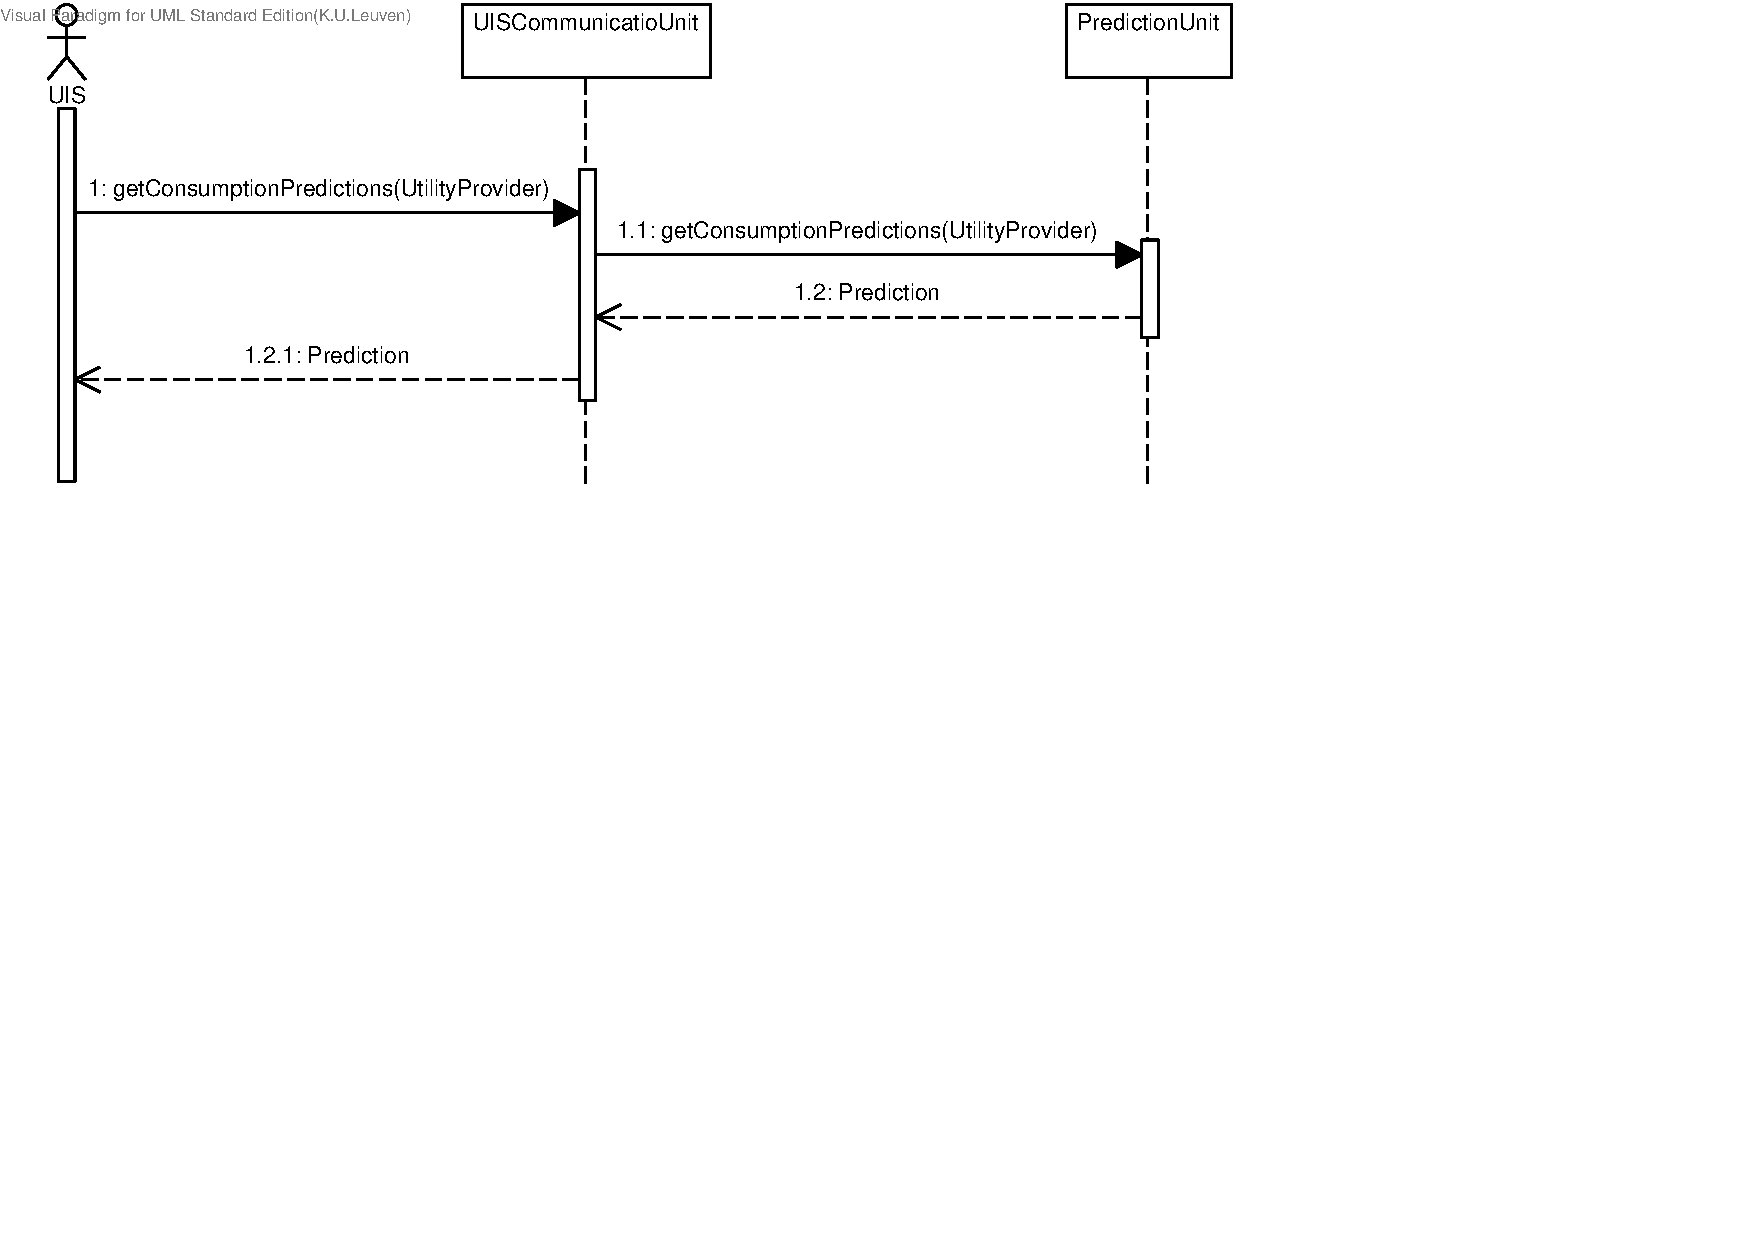
\includegraphics[width=\textwidth]{figs/scenario-5-8.pdf}
		\caption{Sequence diagram for the ``Information exchange towards the UIS''
		scenario}
		\label{fig:scenario-5-8}
	\end{centering}
\end{figure}

\npar Notice that the sequence is started by the UIS in contradiction to the
text in the scenario. The action is inverted because it was stated so in use
case 14 (Request consumption predictions). It is further important to remark
that the inverted situation could easily be modelled in our architecture (but
again this is not done to remain consistent with the use cases).

\npar The consumption demands also can't be retrieved since it was again not
mentioned in any of the use cases. Providing this functionality, however, would
not form a problem at all.
